\section{Session Types}
\label{section:sessiontypes}

Web applications are one of many examples of 
distributed systems in practice. 
Distributed systems are built upon the interaction 
between concurrent processes, which can be implemented using 
the two main communication abstractions in 
\textit{shared memory} and \textit{message passing}. 

Shared memory provides processes with the impression of 
a logical single large monolithic memory 
but requires programmers to understand consistency models 
in order to correctly reason about the consistency of shared state.

Message passing interprets the interaction between processes 
as the exchange of messages.
This best describes the communication transports 
found in web applications, ranging from the 
stateless request-response client-server interactions via HTTP 
to full-duplex communication channels via the WebSocket protocol 
\cite{WebSocketRFC}.

The process algebra $\pi$-calculus 
introduced by Milner in \cite{Milner1999} 
formalises the message passing abstraction in terms of 
the basic building blocks of sending and receiving processes,
along with inductively defined continuation processes. 
The composition of these primitives allow us to 
describe more complex communication sessions.
\textit{Session types} define the typing discipline 
for the $\pi$-calculus and provide reliability guarantees 
for communication sessions; 
the latter addresses a key challenge when 
reasoning about the correctness of distributed systems. 

Practical application of session types in software
engineering range from
developing languages providing native session type support 
\cite{ATS2016} to implementing session types 
in existing programming languages across different paradigms.
Implementations of the latter approach differ by 
how they leverage the design philosophy and features 
provided by the programming language.
For example, King et al. leveraged the 
expressive type system of PureScript to perform 
\textit{static} session type checking in \cite{PureScript2019},
whilst Neykova and Yoshida introduced dynamic approaches to 
check the conformance of Python programs 
with respect to session types in \cite{Python2017}.
We discuss these related work, among others, in \cref{section:bgrelated}.

\subsection{Process Calculus}
\label{subsection:picalculus}

The $\pi$-calculus models concurrent computation, 
where processes can execute in parallel and communicate 
via shared names.
We first consider the \textit{asynchronous} 
$\pi$-calculus introduced by 
Honda and Tokoro in \cite{AsyncHonda}.
Among the many flavours of the calculus 
which vary depending on the application domain,
we outline the variant as presented in \cite{C406Lecture}. 

We define the syntax of processes in \cref{fig:async};
the asynchrony comes from the lack of 
continuation in the output process.

\begin{itemize}
\item $\mathbf{0}$ is the nil process and represents inactivity.
\item $\pout{u}{v}$ is the output process that will send value $v$ on $u$.
\item $\pin{u}{x}.P$ is the input process that,
 upon receiving a message on $u$, 
 will bind the message to $x$ and 
 carry on executing $P$ under this binding.
\item $P\mid Q$ represents the parallel composition of 
processes executing simultaneously.
\item $!P$ represents the parallel composition of 
\textit{infinite} instances of $P$; 
more specifically, $!P \equiv P \mid {!P}$.
\item $(\nu a)~P$ represents a name restriction 
where any occurrence of $a$ in $P$ is local
 and will not interfere with other names outside the scope of $P$.
\end{itemize}

\begin{figure}[!hb]
\doublespacing
\[
\begin{array}{rlr}

P,Q ::= & & \text{Processes} \\
     & \mathbf{0} & \text{Nil Process} \\
\mid & \pout{u}{v} & \text{Output} \\
\mid & \pin{u}{x}.P & \text{Input} \\     
\mid & P \mid Q & \text{Parallel Composition} \\
\mid & !P & \text{Replication} \\
\mid & (\nu a)~P & \text{Restriction} \\

u,v ::= & & \text{Identifiers} \\
     & a, b, c,~\dots & \text{Names} \\
\mid & x, y, z,~\dots & \text{Variables} \\

\end{array}
\]
\singlespacing
\captionof{figure}{Syntax of Asynchronous $\pi$-calculus}
\label{fig:async}
\end{figure}

The operational semantics model the interaction 
between parallel processes. 
Whilst \cite{C406Lecture} presents the full operational semantics, 
we highlight the \rulename{Comm} reduction rule which 
specifically models message passing:
if the parallel composition of an input process and output process 
share the same name, the composition reduces to the 
continuation of the input process, 
substituting the variable $x$ with the message received $v$. 
We omit the definitions of substitution, free variables and free names, 
$\alpha$-equivalence and structural congruence; 
the interested reader may refer to \cite{C406Lecture}.

\begin{prooftree}
\AxiomC{}
\RightLabel{\rulename{Comm}}
\UnaryInfC{$
\pout{a}{v} \mid \pin{a}{x}.P ~\longrightarrow ~ P[v/x]
$}
\end{prooftree}

We additionally define a process $P$ to be {stuck} 
if $P$ is not the nil process and $P$ cannot be reduced any further. 
For example, the process 
$P = \pin{a}{x}.\mathbf{0} \mid \pout{b}{v}$ 
is stuck as the parallel composition of an input process 
and an output process that do not share the same name cannot 
be reduced using \rulename{Comm}. 
In practice, a stuck process contains communications 
that will never be executed.

\subsection{Binary Session Types}
\label{subsection:bgbst}

A \textit{binary session} is a parallel composition 
of two processes, each representing a distinct participant.
In the context of web applications, a binary session may
describe the interactions between client and server.
Without loss of generality, a \text{session} represents 
the sequence of send and receive actions of a single participant.

We introduce a \text{synchronous} session calculus 
in \cref{fig:sync},
inspired by \cite{MPST}. 
We briefly discuss the main components and 
how it differs from the variant introduced in \cite{C406Lecture}:

\begin{itemize}
\item \textbf{Synchronous communication}: 
Output processes have a continuation that will be executed upon
a successful send.

\item \textbf{Polyadic communication}: 
More than one value can be communicated at once.
We refer to these as a \textit{vector} of values, $\vec v$.

\item \textbf{Branching and selection}: 
A branching process can offer a set of branches, 
each defined by its own label identifier and continuation process. 
A selection process can select a branch by 
sending the corresponding label identifier 
alongside the payload to the branching process.

\item \textbf{Labelled messages}: 
A label identifier is attached to all messages; 
the input process in \cref{fig:async}
is generalised as a branching process that offers one branch.
\end{itemize}

The \rulename{Comm} rule in the operational semantics 
for this calculus exemplifies these new additions: 
given a binary session between distinct participants 
$\role{p}$ and $\role{q}$ 
where $\role{q}$ offers a set of labelled branches,
if $\role{p}$ selects a label offered by $\role{q}$ and 
sends a vector of expressions $e_1, \dots, e_n$ 
that evaluate\footnote{
We adopt the operational semantics for 
expression evaluation $e \downarrow v$ 
as defined in \cite{C406Lecture}.
} to the corresponding vector of values 
$v_1, \dots, v_n$, 
the session reduces to a session with 
the continuation from the selection process 
composed with the continuation from the selected branch 
of the branching process.
The branching process binds the received values
$v_1, \dots, v_n$ to the variables $x_1, \dots, x_n$.

\begin{prooftree}
\AxiomC{$\exists	j \in I. l_j = l$}
\AxiomC{$\vec x_j = x_1, \dots, x_n$}
\AxiomC{$e_1 \downarrow v_1 \dots e_n \downarrow v_n$}
\AxiomC{$\mrole{p} \neq \mrole{q}$}
\RightLabel{\rulename{Comm}}
\QuaternaryInfC{$
\mrole{p} :: \sel{q}{l}{e_1 \dots e_n}.~P \mid 
\mrole{q} :: \bra{p}{l_i(\vec x_i): Q_i}{i\in I} 
~\longrightarrow~ 
\ptprocess{p}{P} \mid \ptprocess{q}{Q_j[v_k/x_k]^n_{k=1}}
$}
\end{prooftree}

\begin{figure}[!hb]
\doublespacing
\[
\begin{array}{rlr}
v ::= & \underline{n}~\mid~\texttt{true}~\mid~\texttt{false} 
	& \text{Values} \\
e, e' ::= & & \text{Expressions} \\
	& v & \text{Values} \\
\mid	 & x & \text{Variables} \\
\mid & e + e'~\mid~e - e' & \text{Arithmetic Operators} \\
\mid & e = e'~\mid~e < e' ~\mid~e > e' & \text{Relational Operators} \\
\mid & e \wedge e'~\mid~e \vee e' ~\mid~\neg e & \text{Logical Operators} \\
\mid & e \oplus e' & \text{Non-Determinism} \\

\mrole{p} ::= & \mrole{Client},~\mrole{Server} & \text{Participant} \\

P,Q ::= & & \text{Processes} \\
     & \mathbf{0} & \text{Nil Process} \\
\mid & \sel{p}{l}{\vec e}.~P & \text{Selection} \\
\mid & \bra{p}{l_i(\vec x_i): P_i}{i\in I} & \text{Branching} \\
\mid & \pcond{e}{P}{Q} & \text{Conditional} \\
\mid & \precursion{P} & \text{Recursive Process} \\
\mid & \precvar & \text{Process Variable} \\

l, l' ::= & \texttt{``str''} & \text{Label Identifiers} \\

\mathcal{M} ::= & \ptprocess{p}{P} ~\mid~ \ptprocess{q}{Q} 
	& \text{Binary Session} \\
\end{array}
\]
\singlespacing
\captionof{figure}{Syntax of Session Calculus with 
Branching, Selection and Recursion}
\label{fig:sync}
\end{figure}

Additionally, the calculus introduces:

\begin{itemize}
\item \textbf{Conditionals}: 
If $e \downarrow \texttt{true}$, 
the process $\pcond{e}{P}{Q}$ reduces to $P$; 
if $e \downarrow \texttt{false}$, 
the process $\pcond{e}{P}{Q}$ reduces to $Q$.

\item \textbf{Recursion}: 
Following the \textit{equirecursive} approach, 
the occurrence of the process variable $\precvar$ 
in the recursive process can be 
expanded into the process transparently;
more specifically, $\precursion{P} \equiv P[(\precursion{P})/X]$.
\end{itemize}

{Session types} represent the type theory for our session calculus.
We define the syntax of session types for binary sessions in
\cref{fig:bst}. $\vec U$ denotes a vector of sorts.

\begin{figure}[!hb]
\doublespacing
\[
\begin{array}{rlr}

U ::= & \text{\tt{int}}~\mid~\text{\tt{bool}} & \text{Sorts} \\

T ::= & & \text{Session Types} \\
     & \tend & \text{Termination} \\
\mid & \tbra{p}{l_i(\vec U_i):T_i}{i\in I} & \text{Branching} \\
\mid & \tsel{p}{l_i(\vec U_i):T_i}{i\in I} & \text{Selection} \\
\mid & \trec{T} & \text{Recursive Type} \\
\mid & \trecvar & \text{Type Variable} \\
\end{array}
\]

\singlespacing
\caption{Syntax of Session Types}
\label{fig:bst}
\end{figure}

We derive the type of a process with a {typing judgement} 
of the form $\Gamma \vdash P: S$, which reads, 
\textit{under the typing context $\Gamma$, 
process $P$ has session type $S$}. 

The \textit{typing context} records typing assumptions 
used as part of the derivation: in the case of binary session types, 
the context maps expressions to sorts, 
and process variables to session types. 
A typing judgement is constructed in terms of inference rules 
defined inductively on the structure of 
processes and expressions.

We present the rules for \rulename{Ty-Sel} and \rulename{Ty-Bra}; 
the remaining rules follow from \cite{C406Lecture} 
and can be trivially defined as 
they leverage the syntactic similarities between 
session types and our session calculus.

\begin{prooftree}
\AxiomC{$
\Gamma \vdash e_1 : U_1 ~ \dots ~ \Gamma \vdash e_n : U_n
$}
\AxiomC{$\Gamma \vdash P : T$}
\RightLabel{\rulename{Ty-Sel}}
\BinaryInfC{$
\Gamma \vdash \sel{p}{l}{e_1 \dots e_n}.~P : 
\tselone{p}{l(U_1, \dots, U_n)}: T
$}
\end{prooftree}

\begin{prooftree}
\AxiomC{$
\forall i \in I \left(
\vec x_i = x_1, \dots, x_n
\qquad
\vec U_i = U_1, \dots, U_n
\qquad
\Gamma, x_1: U_1, \dots, x_n: U_n \vdash P_i : T_i
\right)$}
\RightLabel{\rulename{Ty-Bra}}
\UnaryInfC{$
\Gamma \vdash \bra{p}{l_i(\vec x_i): P_i}{i\in I} : 
\tbra{p}{l_i(\vec U_i):S_i}{i\in I}
$}
\end{prooftree}

The definition of stuck processes 
from \cref{subsection:picalculus} 
motivate the discussion of communication errors 
that may occur during interactions among participants. 
We outline two of the main classes of errors:

\begin{itemize}
\item \textbf{Deadlock}: 
Progress cannot be made when the two participants 
expect to be receiving a message from each other at the same time.
\item \textbf{Communication mismatch}: 
Progress cannot be made when the selection process 
sends a message with a label identifier not 
offered by the branching process; 
likewise, the payload sent must be compatible 
with the sort expected by the branching process 
for the selected branch.
\end{itemize}

Session types ensure that 
well-typed binary sessions are guaranteed 
to be free from these communication errors 
through the concept of \textit{duality}. 
Duality defines a notion of \textit{compatibility}
 between processes: two session types are dual 
 with respect to each other if the communication 
 between them (i.e. pairs of sending and receiving actions)
 always match (i.e. with respect to the selected label 
 and message payload type). 
We define $\dual{S}$ as the dual type of $S$ in \cref{table:dual};
message payload types are omitted for brevity.

% Row height in tables
\renewcommand{\arraystretch}{1.6}
\begin{center}
\begin{tabular}{rcl}
$\dual{\tend}$ & = & $\tend$ \\
$\dual{\tbra{p}{l_i: T_i}{i\in I}}$ & = & 
	$\tsel{q}{l_i: \dual{T_i}}{i\in I}$ \\
$\dual{\tsel{p}{l_i: T_i}{i\in I}}$ & = & 
	$\tbra{q}{l_i: \dual{T_i}}{i\in I}$ \\
$\dual{\trec{T}}$ & = & $\trec{\dual{T}}$ \\
$\dual{\trecvar}$ & = & $\trecvar$ \\ 
\end{tabular}
\captionof{table}{Duality of Binary Session Types 
Involving Participants $\role{p}$ and $\role{q}$}
\label{table:dual}
\end{center}
\renewcommand{\arraystretch}{1}

Consequently, a binary session is well-typed 
if the participating processes are typed to be 
dual with respect to each other: 
we illustrate this in \rulename{MTy}.

\begin{prooftree}
\AxiomC{$
\cdot \vdash P : T
$}
\AxiomC{$
\cdot \vdash Q : \dual{T}
$}
\RightLabel{\rulename{MTy}}
\BinaryInfC{$
\vdash \ptprocess{p}{P} \mid \ptprocess{q}{Q}
$}
\end{prooftree}

The definition of duality alone 
restricts the definition of 
well-typed binary sessions to those
where the two processes are derived to be 
\textit{exactly} dual types of one another. 
Consider the pair of session types below:

\[
\begin{array}{rl}
T_{\text{Client}} &= 
	\tselone{Server}{\tmsg{Succ(nat)}}.~
	\tbraone{Server}{\tmsg{Succ(int)}}.~
	\tend \\
T_{\text{Server}} &= \tbraone{Client}{
\begin{cases}
	\tmsg{Succ(int)}: \tselone{Client}{\tmsg{Succ(int)}}. \tend \\
	\tmsg{Quit()}:  \tend \\
\end{cases}
} \\
\end{array}
\]

Whilst $\dual{T_{\text{Client}}} \neq T_{\text{Server}}$, 
this pair of session types is intuitively compatible 
as the client is selecting a branch offered by the server, 
where the session types for the continuations of 
this branch for both participants are indeed dual.
Regarding payload, the server is expecting \texttt{int},
but the client sends \texttt{nat}, which is a subtype of \texttt{int}.

This motivates the concept of \textit{subtypes} in session types,
which allows a process to be typed by its ``supertype'' when required. 
$\subtype$\footnote{
The $\subtype$ operator is also an 
overloaded relation on 
sorts to express subsorting, 
i.e. $\texttt{nat} \subtype \texttt{int}$.
} defines the subtyping relation: 
$T \subtype T'$ reads \textit{$T$ is a subtype of $T'$},
and is defined coinductively on the structure of $T$.

We present the inference rules for 
\rulename{Sub-Sel} and \rulename{Sub-Bra}
inspired by \cite{MPST} but adapted for polyadic communication; 
the intuition behind subtyping and subsorting is outlined below:

\begin{itemize}
\item \textbf{Selection}: 
The supertype of a selection process offers a 
superset of the internal choices and 
can send more generic types of payload; 
intuitively, if a process sends a \texttt{nat}, 
the payload is compatible with receivers expecting 
a more generic \texttt{int} payload.

\item \textbf{Branching}: 
The supertype of a branching process offers 
a subset of the branches and 
expects more specific types of payload; 
intuitively, if a process expects to 
receive an \texttt{int}, 
it can handle a \texttt{nat} payload.
\end{itemize}

\begin{prooftree}
\AxiomC{$\forall i \in I.\left(
\vec U_i = U_1, \dots, U_n 
\quad
\vec U'_i = U'_1, \dots, U'_n
\quad
U_1 \subtype U'_1 ~ \dots ~ U_n \subtype U'_n
\quad
T_i \subtype T'_i
\right)$}
\RightLabel{\rulename{Sub-Sel}}
\doubleLine
\UnaryInfC{$
	\tsel{p}{l_i(\vec U_i):T_i}{i\in I}
	\subtype
	\tsel{p}{l_i(\vec U'_i):T'_i}{i\in I \cup J}
$}
\end{prooftree}

\begin{prooftree}
\AxiomC{$\forall i \in I.\left(
\vec U_i = U_1, \dots, U_n 
\quad
\vec U'_i = U'_1, \dots, U'_n
\quad
U'_1 \subtype U_1 ~ \dots ~ U'_n \subtype U_n
\quad
T_i \subtype T'_i
\right)$}
\RightLabel{\rulename{Sub-Bra}}
\doubleLine
\UnaryInfC{$
	\tbra{p}{l_i(\vec U_i):T_i}{i\in I \cup J}
	\subtype
	\tbra{p}{l_i(\vec U'_i):T'_i}{i\in I}
$}
\end{prooftree}

We also introduce \textit{subsumption} in \rulename{Ty-Sub} 
to incorporate the subtyping relation into the typing judgement.

\begin{prooftree}
\AxiomC{$\Gamma \vdash P: T$}
\AxiomC{$T \subtype T'$}
\RightLabel{\rulename{Ty-Sub}}
\BinaryInfC{$\Gamma \vdash P : T'$}
\end{prooftree}

This allows us to construct a derivation to show that the binary session 

\[
\mathcal{M} = \ptprocess{Client}{P_\text{Client}}
~ \mid ~
\ptprocess{Server}{P_\text{Server}}
\]

is well-typed, assuming $P_\text{Client}$ and $P_\text{Server}$ 
are typed 
$T_\text{Client}$ and $T_\text{Server}$ respectively.

\begin{prooftree}
\AxiomC{\vdots}
\UnaryInfC{$\cdot \vdash P_\text{Client}: T_\text{Client}$}
\AxiomC{\vdots}
\UnaryInfC{$\cdot \vdash P_\text{Server}: T_\text{Server}$}
\AxiomC{\vdots}
\doubleLine
\UnaryInfC{$T_\text{Server} \subtype \dual{T_\text{Client}}$}
\RightLabel{\rulename{Ty-Sub}}
\BinaryInfC{$\cdot \vdash P_\text{Server}: \dual{T_\text{Client}}$}
\RightLabel{\rulename{MTy}}
\BinaryInfC{$
	\vdash \ptprocess{Client}{P_\text{Client}} ~ \mid ~
	\ptprocess{Server}{P_\text{Server}}
$}
\end{prooftree}

\subsection{Multiparty Session Types}
\label{subsection:bgmpst}

Whilst binary session types provide communication guarantees 
between exactly 2 participants, 
distributed systems generally involve more parties in practice. 
This is equally relevant in interactive web applications, 
as motivated by the \textit{Battleships} game example 
in \cite{PureScript2019} where the server coordinates 
interactions between two players. 

Whilst there is a natural syntactical extension to 
our session calculus for 
describing multiparty sessions\footnote{
We also adopt the shorthand 
$\mathcal{M} ::= \prod^n_{i=1} \ptprocess{p_i}{P_i}$ 
as used in the literature.} as

\[
\begin{array}{rl}
\mathcal{M} ::= & \ptprocess{p_1}{P_1} ~\mid~
\ptprocess{p_2}{P_1} ~\mid~\dots~\mid
\ptprocess{p_n}{P_n}
\end{array}
\]

the same cannot be said for the binary session typing discipline,
particularly with respect to duality.
The same notion of duality does not extend to the 
decomposition of multiparty interactions into 
multiple binary sessions: 
\cite{C406Lecture} and \cite{MPST} both present 
counterexamples of well-typed binary sessions that, 
when composed to represent a multiparty session, 
results in communication errors thus 
violating guarantees of well-typed sessions.

Honda et al. presents {multiparty session types} 
in \cite{MPAST} to extend the 
binary session typing discipline for 
sessions involving more than 2 participants, 
whilst redefining the notion of compatibility 
in this multiparty context. 
\textit{Multiparty session types} (MPST)
are defined in terms a \textit{global type},
which provides a bird's eye view of the communication protocol
describing the interactions between pairs of participants. 
\cref{fig:mpst} defines the syntax of global types
inspired by \cite{MPST};
we omit message payload types for brevity.

% Introduce global type, projection
\begin{figure}[!hb]
\doublespacing
\[
\begin{array}{rlr}

G ::= & & \text{Global Types} \\
     & \tend & \text{Termination} \\
\mid & \gcomm{p}{q}{l_i: G_i}{i \in I} & \text{Message Exchange} \\
\mid & \trec{G} & \text{Recursive Type} \\
\mid & \trecvar & \text{Type Variable} \\
\end{array}
\]
\singlespacing
\caption{Syntax of Global Types}
\label{fig:mpst}
\end{figure}

To check the conformance of a participant's process 
against the protocol specification 
described by the global type, 
we \textit{project} the global type onto the participant
to obtain a session type that only preserves the 
interactions described by the global type that 
pertain to the participant. 
Projection is defined by the $\upharpoonright$ operator, 
more commonly seen in literature in its infix form 
as $\proj{G}{p}$ describing the projection of global type 
$G$ for participant $\role{p}$. 
Intuitively, the projected local type of a participant 
describes the protocol from the viewpoint of the participant.

More formally, projection can be interpreted as a 
\textit{partial function} 
${\upharpoonright} :: G \times \mrole{p} \rightharpoonup S$,
as the projection for a participant may be undefined for 
an ill-formed global type; 
\cite{C406Lecture} presents examples of where this is the case, 
and \cite{MPST} presents the formal definition of projection.
We focus on the definition of projection for the 
message exchange global type given below:

\[
\proj{\gcomm{p}{q}{l_i: G_i}{i \in I}}{r} =
\begin{cases}
\tsel{q}{l_i: \proj{G_i}{p}}{i \in I} 
	& \text{if } \mrole{r} = \mrole{p} \\
\tbra{p}{l_i: \proj{G_i}{q}}{i \in I} 
	& \text{if } \mrole{r} = \mrole{q} \\
\underset{i \in I}{\MERGEOP}~\proj{G_i}{r}
	& \text{otherwise} \\
\end{cases}
\]

The third case describes that,
for a participant not involved in the communication,
the projections of the continuations $\proj{G_i}{r}$
do not necessarily have to be the same, but they
need to be ``compatible''. 
The $\mergeop$ syntax denotes the \textit{merging operator}.
It is a partial function on local types allows us to construct
a projection that is compatible with the projections on
the continuations.
We use the \textit{inductive} definition presented by
Scalas and Yoshida in \cite{LessIsMore}, shown in \cref{fig:merge}.

\begin{figure}[!h]
\doublespacing
\[
\begin{array}{rlr}

\tmerge{\tend}{\tend} &= \tend 
	& \rulename{Merge-End} \\
\tmerge{\trecvar}{\trecvar} &= \trecvar 
	& \rulename{Merge-RecVar} \\
\tmerge{\trec{T}}{\trec{T'}} &= \trec{\tmerge{T}{T'}} 
	& \rulename{Merge-Rec} \\
\tmerge{\tsel{p}{l_i: T_i}{i \in I}}{\tsel{p}{l_i: T_i}{i \in I}} 
	&= \tsel{p}{l_i: T_i}{i \in I}
	& \rulename{Merge-Sel} \\
\tmerge{\tbra{p}{l_i: T_i}{i \in I}}{\tbra{p}{l_j: T'_j}{j \in J}} 
	&= \tbra{p}{l_k: T''_k}{k \in I \cup J}
	& \rulename{Merge-Bra} \\

	& 
	\text{where } T''_k =
	\begin{cases}
	T_k & \text{if } k \in (I \setminus J) \\
	T'_k & \text{if } k \in (J \setminus I) \\
	\tmerge{T_k}{T'_k} & \text{otherwise} \\
	\end{cases}
	& \\

\end{array}
\]
\singlespacing
\captionof{figure}{Definition of Merging Operator}
\label{fig:merge}
\end{figure}

The notion of compatibility in multiparty session types 
is still captured by \rulename{MTy}, 
but adapted to consider the local projections for 
all participants as supposed to dual types in the binary case. 

\begin{prooftree}
\AxiomC{$
\forall i \in I. ~ \left( \cdot \vdash P_i : \proj{G}{p_i} \right)
$}
\AxiomC{$
\pt{G} \subseteq \left\{ \mrole{p_i} \mid i \in I \right\}
$}
\RightLabel{\rulename{MTy}}
\BinaryInfC{$
\displaystyle \vdash \prod^{}_{i \in I} \ptprocess{p_i}{P_i} ~: G
$}
\end{prooftree}

For a multiparty session 
$\mathcal{M} = \prod_{i \in I} \ptprocess{p_i}{P_i}$ 
to be well-typed by a global type $G$: 

\begin{enumerate}
\item 
All participant processes $\mrole{p_i}{P_i}$ are well-typed 
with respect to their corresponding well-defined projection 
$\proj{G}{p_i}$, and 
\item 
$G$ does not describe interactions with participants 
not defined in $\mathcal{M}$.
$\pt{G}$ denotes the set of participants in the global type $G$,
defined inductively on $G$ as shown on \cref{table:pt}.

\renewcommand{\arraystretch}{1.6}
\begin{table}[!h]
\centering
\begin{tabular}{rcl}
$\pt{\tend}$ &=& $\emptyset$ \\
$\pt{\trecvar}$ &=& $\emptyset$ \\
$\pt{\trec{G}}$ &=& $\pt{G}$ \\
$\pt{\gcomm{p}{q}{l_i: G_i}{i \in I}}$ &=& 
	$\{ \mrole{p}, \mrole{q} \} \cup \underset{i \in I}{\bigcup}~\pt{G_i}$
	\\
\end{tabular}
\captionof{table}{Definition of Participants in Global Types}
\label{table:pt}
\end{table}
\renewcommand{\arraystretch}{1}

\end{enumerate}

Well-typed multiparty sessions enjoy the following 
communication guarantees as outlined in \cite{GentleMPST}:

\begin{itemize}
\item \textbf{Communication safety}: 
The types of sent and expected messages will always match.
\item \textbf{Protocol fidelity}: 
The exchange of messages between processes will abide by the global protocol.
\item \textbf{Progress}: 
Messages sent by a process will be eventually received, 
and a process waiting for a message will eventually receive one; 
this also means there will not be any sent but unreceived messages.
\end{itemize}

This motivates an elegant, decentralised solution for 
checking protocol conformance in practice: 
once the global type for the protocol is defined, 
local processes can verify their implementation 
against their corresponding projection in isolation, 
independent of each other. 
We illustrate this in \cref{fig:mpstworkflow}.

\begin{figure}[!ht]
\centering
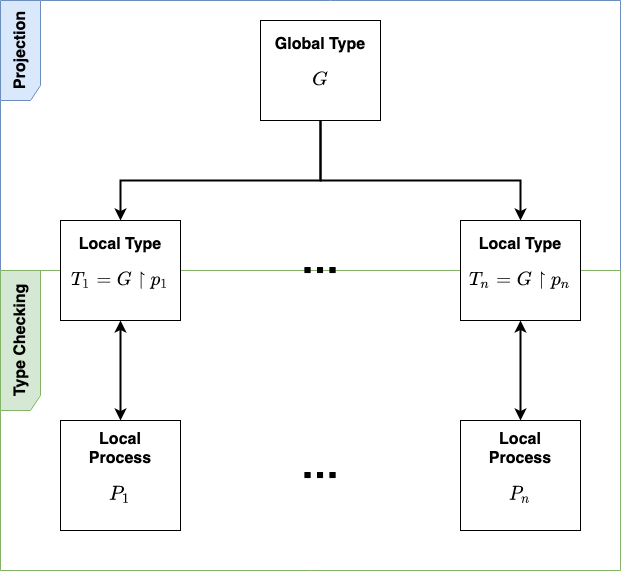
\includegraphics[width=.75\textwidth]{MpstFramework}
\caption{Type Checking with Multiparty Session Types}
\label{fig:mpstworkflow}
\end{figure}